% \documentclass{standalone}
% \input{../tikz_header}

% \begin{document}

 
 
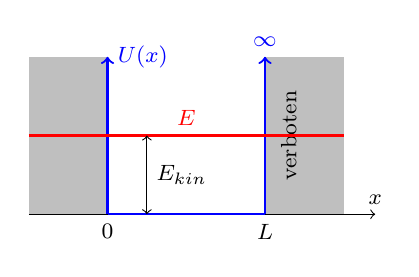
\begin{tikzpicture}[font=\footnotesize]

  \fill[gray!50!white] (-1,0) rectangle (-2,2);
  \fill[gray!50!white] (1,0) rectangle (2,2);

  \draw[->](-2,0) -- (2.4,0) node [above] {$x$};
  \node[ rotate=90] at (1.3,1) {verboten};

  \node[below] at (-1,0) {$0$};
  \node[below] at (1,0) {$L$};

  \draw[thick, blue, ->]  (-1, 0) -- (-1, 2) node [right ] {$U(x)$};
  \draw[thick, blue, ->]   (1, 0) -- (1, 2) node[above] {$\infty$};
  \draw[thick, blue] (-1, 0) -- (1, 0);

  \draw[thick, red] (-2,1) -- node[above]{$E$} (2, 1);
  \draw[<->] (-0.5, 0) --node[right]{$E_{kin}$} (-0.5, 1);


\end{tikzpicture}


%\end{document}


